\section{Introducción}
\label{IntroduccionConcurrencia}

``La idea de programación concurrente siempre estuvo asociada al mundo de los
\textit{Sistemas Operativos}. No en vano, los primeros programas concurrentes
fueron los propios Sistemas Operativos de multiprogramación en los que un solo
procesador debía repartir su tiempo entre muchos usuarios.''\cite{PalmaConcurrente}

En las últimas dos décadas, la programación concurrente ganó gran interés y
actualmente está presente en la mayoría de las aplicaciones.
Esto se debe principalmente a algunos grandes hitos en la programación:
\begin{itemize}
	\item La generalización del concepto de \textit{hilo} o \textit{thread}.
	Permiten la ejecución de programas de manera más rápida y eficiente que los programas
	basados en procesos.
	\item La disponibilidad de lenguajes de alto nivel con soporte para
	programación de hilos y de procesos.
	\item Los entornos de internet, donde la concurrencia se hace necesaria
	en todo aspecto.
	\item El desarrollo y gran avance de hardware capaz de ejecutar múltiples hilos
	y procesos de forma paralela. Esto permite aprovechar las ventajas de
	performance de la concurrencia. Las principales arquitecturas capaces de
	explotar el paralelismo a nivel de hilo y/o de proceso son
	\begin{itemize}
	    \item Procesadores Multi-Core
	    \item Procesadores Many-Core
	    \item Procesadores con soporte Multi-Thread
    \end{itemize}
\end{itemize}

\section{Programación Concurrente}
\label{ProgramacionConcurrente}

La \textit{programación concurrente} es la disciplina que se encarga del estudio
de las notaciones que permiten especificar la ejecución concurrente de las
acciones de un programa, así como resolver los problemas inherentes a la
ejecución concurrente (ver \ref{ProblemasConcurrencia}). Es de interés
formalizar el concepto de ejecución concurrente y de ejecución paralela a fin
de poder diferenciarlos:

\begin{itemize}
	\stepcounter{definitionsCounter}
	\item \underline{Definición \thedefinitionsCounter :}  Dos hilos
	\footnote{En adelante, se hablará de concurrencia de hilos dado que los
	sistemas de referencia son de memoria compartida. En el caso que corresponda
	hablar de procesos se lo mencionará explícitamente.} son \textit{concurrentes}
	si la primera instrucción de uno de ellos se ejecuta después de la primera del
	otro y antes de la última.
	\stepcounter{definitionsCounter}
	\item \underline{Definición \thedefinitionsCounter :}  Dos hilos 	se están
	ejecutando de manera \textit{paralela} si son concurrentes y la ejecución de
	ambos se da al mismo tiempo.
\end{itemize}

Para que dos hilos sean concurrentes no es necesario que se ejecuten al mismo
tiempo, es suficiente que exista un intercalado entre la ejecución de sus
instrucciones \cite{PalmaConcurrente}. En este proyecto integrador, es de
interés fundamentalmente la ejecución concurrente.

Anteriormente en esta sección se mencionó que existen problemas aparejados a la
programación de sistemas concurrentes. Sabiendo esto resulta necesario conocer
las ventajas de la programación concurrente, que justifiquen su uso por encima de
las dificultades que genera.

\subsection{Ventajas de la Programación Concurrente}

Los beneficios de programar de manera concurrente se engloban en tres
categorías:

\begin{itemize}
	\item \underline{Incremento en la velocidad de ejecución:} Cuando se ejecuta un
	programa concurrente en un entorno multiprocesador, los distintos hilos que
	lo forman se ejecutan de manera paralela, con lo que el tiempo total de
	ejecución se reduce. Esto es especialmente ventajoso en programas de cálculo
	numérico.
	\item \underline{Solución de problemas inherentemente concurrentes:} Existen
	problemas cuya naturaleza es concurrente, por lo que un modelo de programación
	de este tipo se adapta más naturalmente a la resolución de estos problemas.
	\item \underline{Mejor aprovechamiento del tiempo de CPU:} Un sistema operativo
	con un ambiente de multiprogramación que permita la concurrencia es capaz de
	desalojar a un hilo que está esperando por un evento y no está haciendo uso
	de la CPU para brindarle este tiempo a otro hilo que lo requiera.
\end{itemize}

\subsection{Problemas y Propiedades de la Concurrencia}
\label{ProblemasConcurrencia}

Como se introdujo en la sección \ref{ProgramacionConcurrente}, existen
problemas que aparecen al programar de manera concurrente. Esto lleva a que los
programas concurrentes deban satisfacer una serie de propiedades (además de su
especificación técnica del dominio del problema) para funcionar correctamente.

Estas propiedades se dividen en dos grupos:

\subsubsection*{Propiedades de Seguridad}
Las propiedades de seguridad aseguran que ``nada malo'' va a pasar en la
ejecución del programa \cite{PalmaConcurrente}.
Estas son:

\begin{itemize}
    \item \underline{Exclusión Mutua:} Existen recursos que no deben ser
    accedidos concurrentemente para evitar problemas de coherencia y
    consistencia. Por esto se debe garantizar que a lo sumo un hilo está
    accediendo a un recurso de este tipo en un instante dado.
    \item \underline{Condición de Sincronización:} Existen situaciones
    donde un hilo debe esperar la ocurrencia de un evento para continuar su
    flujo. Ante estos casos se debe garantizar que el hilo espere por dicha
    ocurrencia, de otro modo el resultado puede ser indefinido o inesperado.
    \item \underline{Interbloqueo \textit{(Deadlock)}:} Sucede cuando dos o más
    hilos están esperando a que suceda un evento que nunca ocurrirá para
    continuar sus flujos de ejecución. El evento no ocurre porque las
    condiciones para que suceda están bloqueadas por los propios hilos.\\
    Para que el interbloqueo suceda efectivamente se tienen que cumplir las
    siguientes condiciones:
    \begin{itemize} 
        \item Exclusión Mutua: si no se exige exlusión mutua, no puede haber
        interdependencia entre los hilos.
        \item Retención y Espera: cada hilo debe retener un recurso y esperar
        a que se libere otro.
        \item No Apropiación: no se puede forzar a un hilo a que desaloje un
        recurso
        \item Circulo Vicioso de Espera: Se forma una cadena cerrada de
        solicitudes, donde cada hilo retiene al menos un recurso que necesita el
        próximo hilo.
    \end{itemize}
    Las tres primeras condiciones son necesarias pero no suficientes para que
    efectivamente ocurra el interbloqueo. La cuarta condición nace como
    consecuencia de las tres primeras, siempre que se produzca una secuencia de
    eventos que desemboque en un círculo de espera irresoluble
    \cite{SistOpStallings}.
\end{itemize}

\subsubsection*{Propiedades de Vivacidad}

Si se aseguran las propiedades de vivacidad, ``algo bueno'' pasará eventualmente
en la ejecución del programa.

\begin{itemize}
    \item \underline{Interbloqueo Activo \textit{(Livelock)}:} Se produce un
    interbloqueo activo cuando un sistema ejecuta una serie de instrucciones sin
    hacer ningún progreso. Esto se da cuando $N$ hilos necesitan $N$ recursos
    y se los intercambian sin obtener nunca el conjunto completo.
    \item \underline{Inanición \textit{(Starvation)}:} Ocurre cuando al menos
    una parte del sistema nunca recibe los recursos necesarios para
    continuar, o los recibe demasiado tarde para lograr el resultado
    esperado. No es necesario que todo el sistema se bloquee para estar en una
    situación de inanición.
\end{itemize}

\section{Mecanismos de Sincronización}

A fin de garantizar el cumplimiento de las propiedades introducidas en la
sección \ref{ProblemasConcurrencia}, es necesario sincronizar la ejecución de
los hilos. De lo contrario, emergen problemas de coherencia y/o consistencia de
datos, o corrupción.

\subsection{Cooperación vs Competencia}

La sincronización de hilos se implementa basada en dos principios
\cite{SistOpStallings}:
\begin{itemize}
    \item \underline{Cooperación:} Los hilos se comunican entre ellos para
    cooperar en la compartición de recursos. A su vez, existen dos tipos de
    cooperación:
    \begin{itemize}
        \item \underline{Cooperación por Compartición:} Los hilos interactúan
        para gestionar los recursos. No tienen conocimiento explícito de los demás.
        \item \underline{Cooperación por Comunicación:} Los hilos interactúan
        para gestionar los recursos mediante el paso explícito de mensajes entre
        ellos.
    \end{itemize}
    \item \underline{Competencia:} Los hilos compiten entre sí por los
    recursos. La gestión de los recursos se efectúa por otra entidad, como el
    sistema operativo.
\end{itemize}

\subsubsection{Cooperación por Compartición de Recursos}

Los hilos inteactúan entre ellos sin tener conocimiento explícito de la
existencia de los demás.

Existen regiones de almacenamiento de datos compartidas (espacios de memoria,
archivos, bases de datos, etc), accedidas por múltiples hilos.

Si bien un hilo no hace referencia a ningún otro, es consciente de que los
datos compartidos son accedidos y modificados por los demás. Por lo que
el conjunto debe cooperar para asegurar que los datos compartidos se gestionen
correctamente. Es responsabilidad de los mecanismos de control asegurar la
integridad de los datos compartidos \cite{SistOpStallings}.

Como los datos se almacenan en recursos compartidos, existen los problemas de
exclusión mutua, interbloqueo e inanición vistos en la sección
\ref{ProblemasConcurrencia}. La principal diferencia es que existen dos modos de
acceder a los datos: para \textit{lectura} y para \textit{escritura}. Únicamente
se debe asegurar la exclusión mutua para operaciones de escritura ya que son las
únicas capaces de romper la \textit{coherencia} y \textit{consistencia} de los
datos.

Un conjunto de datos son coherentes si independientemente de quién haya sido el
último escritor, cualquier lector obtiene el último conjunto de valores escrito.
Por otro lado, un dato es consistente si un lector obtiene un valor que fue
realmente escrito por un escritor y no un dato corrupto.

Algunos mecanismos para gestionar el uso de los datos compartidos son:
\begin{itemize}
    \item Semáforos: desarrollado en la sección \ref{semaforos}
    \item Monitores: desarrollado en la sección \ref{monitores}
\end{itemize}

\subsubsection{Cooperación por Comunicación entre Hilos o Procesos}

Cuando los hilos o procesos cooperan por comunicación, participan en alcanzar un
objetivo en común. La comunicación es una manera de sincronizar o coordinar las
distintas actividades.

La comunicación está formada por está formada por el emisor, el receptor, el
canal y el mensaje. El envío y recepción de mensajes son explícitos.
Las herramientas para este paso de mensajes están dadas por el lenguaje de
programación, alguna biblioteca o por el sistema operativo.

Al no haber compartición de datos entre los hilos o procesos, no es necesaria la
ejecución en exclusión mutua. Pese a esto, el interbloqueo y la inanición siguen
siendo problemas que pueden afectar a los hilos o proceos
\cite{SistOpStallings}.

\subsubsection{Competencia entre Hilos}

Los hilos no tienen forma de comunicarse entre ellos para gestionar los
recursos.

Si dos hilos desean acceder a un mismo recurso, el sistema operativo se lo
asignará a uno de ellos y el otro tendrá que esperar. Se debe garantizar:
\begin{itemize}
    \item La toma de los recursos en exlusión mutua.
    \item Correcta gestión de los recursos para evitar interbloqueos.
    \item La reactivación de los hilos bloqueados en un tiempo prudente a fin de
    evitar su inanición.
\end{itemize}
El control de la competencia involucra al sistema operativo
inevitablemente, porque es él quien asigna los recursos del sistema.
Además, los hilos deben ser capaces por sí mismos de expresar de algún
modo los requisitos de exclusión mutua, como puede ser bloqueando los
recursos antes de usarlos. Cualquier solución conlleva alguna ayuda del
sistema operativo, como la provisión del servicio de
bloqueo.\cite{SistOpStallings}

\begin{framed}
\textbf{Nota:} A los fines de este proyecto integrador sólo es de interés la
concurrencia basada en memoria compartida. Dentro de este modelo se destacan dos
mecanismos de sincronización por competencia: los \textit{semáforos} y los
\textit{monitores}.
\end{framed}

\subsection{Semáforos}
\label{semaforos}

Los semáforos fueron el primer mecanismo de sincronización de hilos por
cooperación. Fueron desarollados por E. Dijkstra en 1965 como mecanismos
eficientes y fiables para dar soporte a la cooperación de hilos en un sistema
operativo.

El principio en el que se basan es simple. Un conjunto de hilos pueden
cooperar utilizando señales, de manera que se pueda obligar a un hilo a
detener su ejecución en un punto específico hasta recibir una señal conocida.
La señalización está a cargo de los semáforos.

Para transmitir una señal sobre el semáforo $s$, el hilo $p$ debe ejecutar
$signal(s)$, y para recibir una señal de $s$, debe ejecutar $wait(s)$. Si la
señal no fue transmitida, $p$ se bloquea hasta recibir la señal.

Efectivamente, las operaciones sobre los semáforos son tres:
\begin{itemize}
    \item \underline{$init(sem\ s,\ uint\ n)$:} inicializa al semáforo $s$ con
    un entero positivo $n$.
    \item \underline{$wait(sem\ s)$:} decrementa el valor del semáforo. Si se
    hace negativo, el hilo que realiza la llamada se bloquea. También se la
    llama \textit{acquire}.
    \item \underline{$signal(sem\ s)$:} incrementa el valor del semáforo. Si
    había un hilo bloqueado por una llamada a $wait(s)$, se desbloquea. También
    se la llama \textit{release}.
\end{itemize}

Las llamadas a $signal(s)$ y $wait(s)$ son atómicas para asegurar la
modificación del contador del semáforo en eclusión mutua.

Los hilos que esperan una señal luego de bloquearse por una llamada a
$wait(s)$ deben hacerlo en una cola de espera. Esta cola implementa una política
que decide cuál hilo bloqueado se libera ante la llegada de una señal. El
caso más típico es FIFO, pero se puede implementar otro. Sea cual fuera la
política implementada, se debe asegurar que ningún hilo bloqueado sufrirá
inanición por ella.

Los semáforos descriptos hasta este punto son de tipo \textit{semáforo
general}.
Existe una versión más reducida que sólo puede adquirir valores $0$ y $1$ llamada
\textit{semáforo binario}. Los semáforos binarios son de implementación más
simple que los generales y se demuestra que tienen la misma potencia de
expresividad. \cite{SistOpStallings}

\subsection{Monitores}
\label{monitores}

Los semáforos son herramientas simples y potentes para la gestión de la
concurrencia. Permiten gestionar la ejecución en exclusión mutua y coordinar
hilos. El problema de los semáforos radica en que las operaciones signal(s)
y wait(s) están distribuidas por el código de todos los hilos que lo usan,
con lo que resulta muy difícil entender y predecir el efecto de una operación
sobre todos los hilos que dependen del mismo semáforo.

Para solucionar este problema, C. Hoare definió el concepto de monitor en su
artículo “Monitors: An Operating System Structuring Concept.” en 1974.

Los monitores, al igual que los semáforos, son herramientas de gestión de la
concurrencia entre hilos. Los hilos los usan para asegurar el acceso en
exclusión mutua a recursos y para sincronizar y comunicarse con otros
hilos.\\
El propósito de un monitor de concurrencia es centralizar la gestión de los
recursos compartidos en una sección del código del programa. De esta manera, la
responsabilidad de sincronizar a los hilos para evitar problemas de concurrencia
es enteramente del monitor y no de cada hilo que quiera acceder a un recurso.

Un monitor consiste en un grupo de datos y un conjunto de rutinas exportadas
(llamadas \textit{rutinas de entrada}). Estas rutinas realizan operaciones sobre
los datos. Los datos del monitor representan recursos compartidos para múltiples
hilos (ya sean de software o de hardware) y pueden ser modificados únicamente
dentro de las rutinas del monitor.

La forma que tiene un monitor de gestionar concurrencia es:
\begin{itemize}
    \item Asegurando la ejecución de sus rutinas en exclusión mutua.
    \item Gestión de los recursos de forma implícita o explícita
\end{itemize}

Para asegurar la ejecución en exclusión mutua, sólo se permite que un único
hilo pueda ejecutar una rutina del monitor a la vez. Este hilo recibe el
nombre de \textit{hilo activo}. El hilo activo bloquea la entrada al
monitor cuando ejecuta una rutina y la desbloquea cuando cede
\textit{voluntariamente} el control del monitor. Si otro hilo llama a una
rutina de entrada mientras el monitor está bloqueado, se bloquea en una cola de
entrada al monitor hasta que este pase a estado desbloqueado.

\subsubsection{Sincronización Explícita}
\label{monitor_sincronizacion_explicita}

En muchas ocasiones resulta necesario no sólo garantizar la exclusión mutua
dentro del monitor sino sincronizar hilos dentro de él para la correcta
gestión de los recursos compartidos (cola de cortesía). Para esto el monitor
representa los recursos con variables de condición (o colas de eventos)

\begin{framed}
\paragraph{Variables de condición:} \label{variables_condicion} Son variables
especiales, sobre las que se pueden realizar dos acciones:
\begin{itemize}
    \item delay: Suspende al hilo que la llama, a la espera de una señal.
    \item signal: Levanta el estado de suspensión de un hilo suspendido por
    una llamada a \textit{delay()} sobre ella. Si no hay ningún hilo
    suspendido no tiene efecto.
\end{itemize}
Si existe más de un hilo suspendido en una variable de condición cuando otro
hace una llamada a \textit{signal()}, el hilo a despertar será elegido
aplicando una política determinada. Esta política puede ser FIFO, por
prioridades por hilo, etc.
\end{framed}

El hilo activo del monitor puede suspenderse a sí mismo temporalmente bajo
una condición x ejecutando \textit{delay(x)}. Al suspenderse deja de ser el
hilo activo y se sitúa al final de la cola de la condición x, a la espera de
volver a entrar al monitor cuando la condición cambie. Previo a esto debe
desbloquear la entrada al monitor para no generar un interbloqueo con los demás
hilos que intentan acceder. Por otro lado, otro hilo que sea el activo
puede hacer una llamada a \textit{signal(x)} si detecta un cambio en \textit{x},
desbloqueando un hilo suspendido en su cola de condición asociada.

Es común asociar una variable de condición a una proposición lógica sobre el
estado de un recurso gestionado por el monitor, por ejemplo “El buffer A no
está lleno”. De esta manera esperar por esta condición equivale a esperar a que
el buffer A no esté lleno. Esta asociación suele ser implícita, es decir que le
da semántica al monitor pero no forma parte de su funcionamiento.

\subsubsection{Sincronización Implícita}

Como alternativa a la señalización manual, Hoare propone los monitores de
señalización automática. Este tipo de monitor elimina las variables de
condición modificando la directiva \textit{wait} para que reciba una proposición
lógica.

Un hilo que llame \textit{wait(prop)} se mantiene bloqueado mientras la
proposición \textit{prop} sea falsa. Cuando \textit{prop} cambie a ser
verdadera, los hilos que estén bloqueados se desbloquean automáticamente.
Un inconveniente con este mecanismo es que su implementación suele llevar a la
señalización repetida de muchos hilos, con los consecuentes cambios de contexto.

A los efectos de este proyecto integrador, es de mayor interés el monitor de
sincronización explícita. Por esto, los siguientes apartados al respecto son
referidos únicamente a este tipo de monitor.

\subsubsection{Estructura de un Monitor}
De forma general, un monitor de concurrencia de sincronización explícita está
compuesto por las siguientes partes:
\begin{itemize}
    \item Variables de condición
    \item Colas de condición
    \item Rutinas exportadas o de entrada
    \item Cola de entrada
    \item Cola de espera
    \item Cola de cortesía o del señalizador
\end{itemize}

En la figura \ref{fig:monitor01} se observa la estructura de un monitor de
concurrencia:

\begin{figure}[H]
  \centering
  \makebox[\textwidth][c]{
    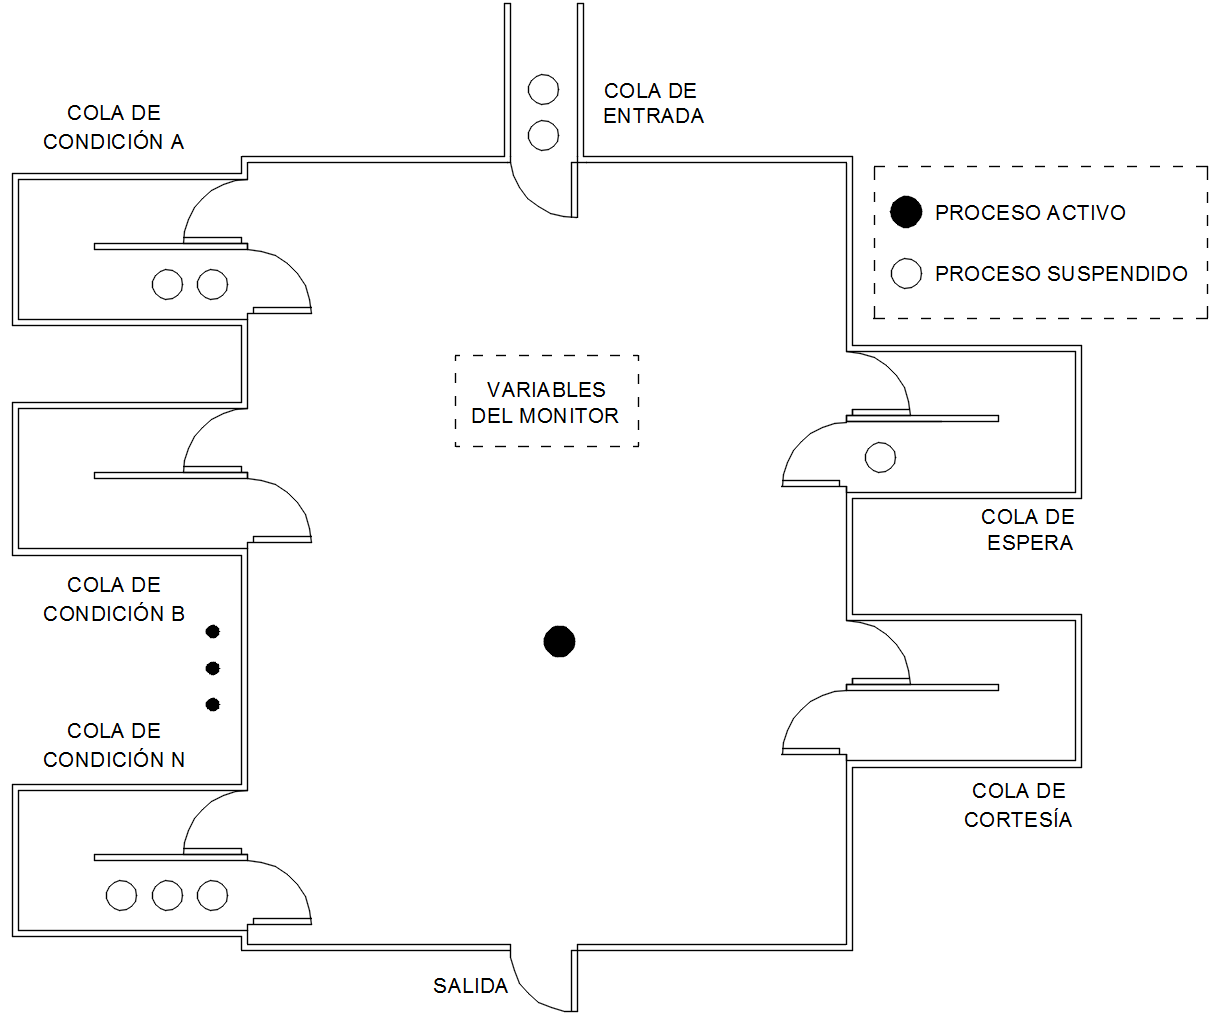
\includegraphics[width=140mm]{Monitor}
  }
  \caption{Estructura de un Monitor de Concurrencia}
  \label{fig:monitor01}
\end{figure}

Aunque un hilo puede entrar al monitor llamando a cualquiera de sus
procedimientos expuestos, y puesto que se debe asegurar la ejecución en
exclusión mutua se puede considerar que existe un único punto de entrada al
monitor. De ahí que existe una única cola de entrada.

\subsubsection{Máquina de Estados de un Monitor}
Un monitor no es un proceso en sí mismo, por lo que no tiene un hilo de
ejecución. En su lugar, es ejecutado por los hilos de los procesos que llaman a
alguna de sus rutinas.

El estado del monitor, incluyendo si está o no bloqueado determina si un
hilo que intenta ejecutar una rutina de entrada puede continuar o si se bloquea.

Se puede representar el funcionamiento de un monitor por dos máquinas de
estado. La primera indica si el monitor está bloqueado o desbloqueado. La
segunda representa el estado de las colas del monitor.
\begin{itemize}
    \item Estados del Primer Autómata:
    \begin{itemize}
        \item Bloqueado: Un hilo está ejecutando una rutina del monitor
        \item Desbloqueado: No hay hilo activo en el monitor
    \end{itemize}
    \item Estados del Segundo Autómata: Las colas que influyen en el estado del
    monitor son las internas a este (las de condición, la de espera y la de
    cortesía). La cola de entrada no influye en el estado del monitor porque no
    refleja la situación interna del mismo.\\
    Como los estados que puede adquirir una cola son \textit{“vacía”} y
    \textit{“no vacía”}, los estados del segundo autómata son todas las
    combinaciones posibles de las tres colas internas del monitor en cada uno de
    sus estados.
\end{itemize}

\begin{figure}[H]
  \centering
  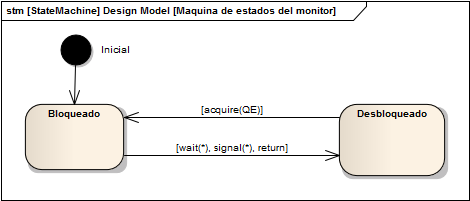
\includegraphics[width=100mm]{Primer_Automata_Monitor}
  \caption{Primer Autómata de un Monitor de Concurrencia}
  \label{fig:automata_monitor01}
\end{figure}

\begin{figure}[H]
  \centering
  \makebox[\textwidth][c]{
    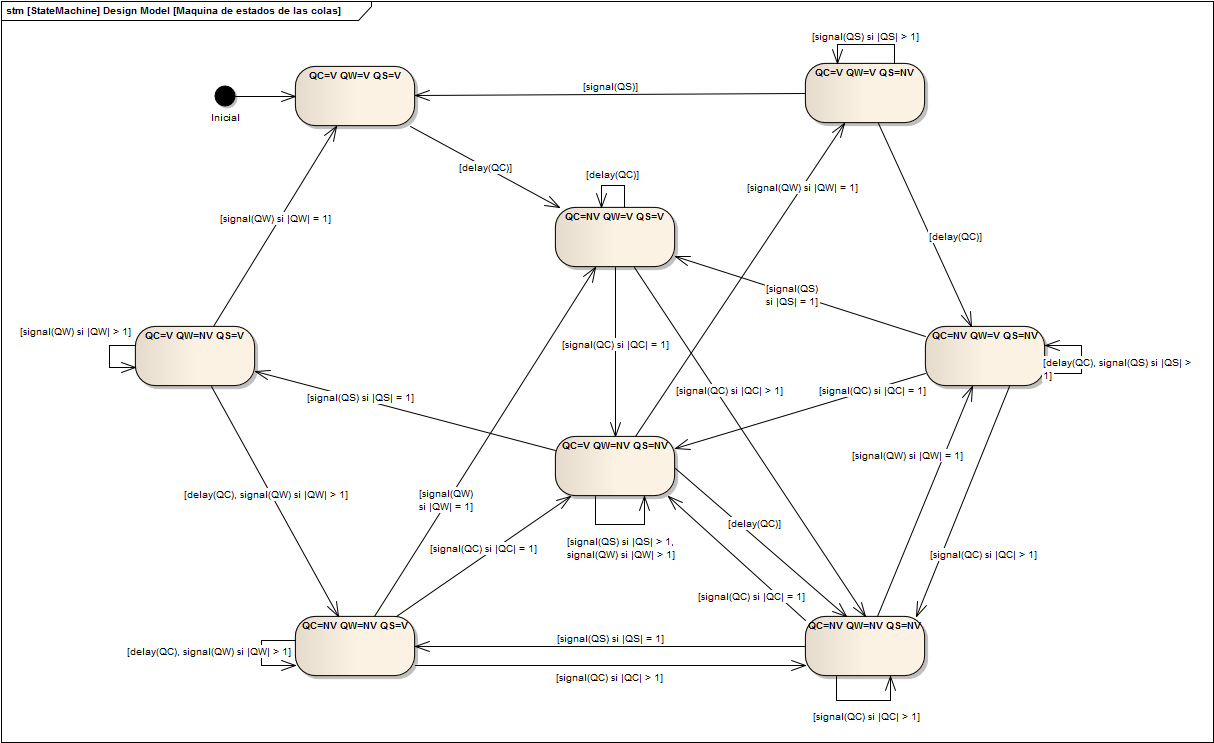
\includegraphics[width=\textwidth]{Segundo_Automata_Monitor}
  }
  \caption{Segundo Autómata de un Monitor de Concurrencia}
  \label{fig:automata_monitor02}
\end{figure}

\begin{framed}
\textbf{Nota:} Como se explicó en la sección \ref{comparacion_rdp_automatas} se
puede obtener un único autómata a partir de estos dos, pero es de la opinión de los autores
que esto resultaría en una explicación más confusa.
\end{framed}

\subsubsection{Políticas de Desbloqueo de Hilos}
\label{politica_monitor}
El desbloqueo de un hilo suspendido en la cola de condición x debe ser hecho
por el hilo que produjo el cambio sobre esta condición. La siguiente acción a
realizar luego del desbloqueo dependerá del tipo de monitor en cuestión.
Se puede generar una clasificación de monitores basándose en el comportamiento
luego del desbloqueo de un hilo. A continuación se presentan los tipos de
monitores introducidos en \cite{PalmaConcurrente}

\begin{framed}
\textbf{Nota:} Para todos los siguientes casos, se considera que el hilo
\textit{A} desbloquea al hilo \textit{B} ejecutando \textit{signal(x)},
condición sobre la que \textit{B} se encuentra bloqueado inicialmente. Por lo
tanto, al comenzar cada párrafo, A está bloqueado en la cola de cortesía y B en
la de espera, a menos que se indique lo contrario.
\end{framed}

\paragraph{Desbloquear y continuar (Signal and Continue)}
Se desbloquea a \textit{A} de la cola de cortesía y continúa su ejecución dentro
del monitor, ya sea hasta terminar la llamada al procedimiento o hasta bloquearse
en una cola de condición. Una vez \textit{A} sale del monitor, \textit{B}
ejecuta la instrucción siguiente al \textit{delay(x)} que lo bloqueó. En este
punto, \textit{B} debe volver a verificar la condición que lo suspendió porque
no se puede garantizar que \textit{A} no la haya modificado luego de la llamada
a \textit{signal(x)}.

\paragraph{Retorno forzado}
Se desbloquea a \textit{A}, quien ejecuta una instrucción de salida del monitor
(\textit{return} o \textit{delay(n)}) justo después. De esta manera, no es
necesario que \textit{B} vuelva a comprobar su condición ya que la exclusión
mutua asegura que no fue modificada.


\paragraph{Desbloquear y esperar}
\textit{A} está en la cola de entrada del monitor en lugar de la de cortesía.\\
Se desbloquea a \textit{B} de la cola de espera para que continúe su ejecución
en el monitor. Este enfoque tiene la ventaja de que \textit{B} no necesita
comprobar su condición de bloqueo una vez desbloqueado, pero \textit{A} cede su
lugar en el monitor y debe volver a competir por el ingreso para poder terminar
su ejecución.


\paragraph{Desbloquear y espera urgente}
Esta política soluciona el problema de inequidad de \textit{Desbloquear y
Esperar}.\\
Se desbloquea a \textit{B}, pero \textit{A} se suspende en la cola de cortesía.
De esta manera, el desbloqueo de \textit{A} tendrá prioridad sobre cualquier
hilo que intente entrar al monitor.

\paragraph{Clasificación Generalizada de Políticas de Desbloqueo:}
En \cite{MonitorClassification} el autor hace un análisis más exhaustivo de las
posibilidades existentes para diseñar una política de desbloqueo de hilos.
Dadas las tres colas de donde se puede elegir un hilo para desbloquear se
plantea una prioridad para cada una, resultando en:
\begin{itemize}
    \item EP: prioridad de la cola de entrada (entry queue priority)
    \item WP: prioridad de la cola de espera (waiting queue priority)
    \item SP: prioridad de la cola de cortesía (signaler queue priority)
\end{itemize}
Asignando pesos relativos a las tres prioridades se llega a que existen 13
distintas posibilidades.

En la tabla \ref{tab:prioridades_monitores} se Enumeran las posibilidades. La
tercera columna se refiere a los monitores definidos en [Howard, J. "Proving
Monitors"]

\begin{table}[H]
\centering
\begin{tabular}{|c|c|c|}
\hline
 & Prioridades relativas & Monitor Tradicional Correspondiente \\ \hline
1 & $EP = WP = SP$ & Random\\ \hline
2 & $EP = WP < SP$ & Wait and Notify\\ \hline
3 & $EP = SP < WP$ & Signal and Wait\\ \hline
4 & $EP < WP = SP$ & \\ \hline
5 & $EP < WP < SP$ & Signal and Continue\\ \hline
6 & $EP < SP < WP$ & Signal and Urgent Wait\\ \hline
7 & $EP > WP = SP$ & RECHAZADO\\ \hline
8 & $EP = SP > WP$ & RECHAZADO\\ \hline
9 & $SP > EP > WP$ & RECHAZADO\\ \hline
10 & $EP = WP > SP$ & RECHAZADO\\ \hline
11 & $WP > EP > SP$ & RECHAZADO\\ \hline
12 & $EP > SP > WP$ & RECHAZADO\\ \hline
13 & $EP > WP > SP$ & RECHAZADO\\ \hline
\end{tabular}
\caption{Tipos de monitores según las prioridades relativas de sus colas}
\label{tab:prioridades_monitores}
\end{table}

Las propuestas 7 a 13 son rechazadas porque si la prioridad de entrada es mayor
que cualquiera de las otras dos, ante un flujo constante de hilos de
entrada, habría al menos una cola que nunca sería atendida, lo que lleva a
posible inanición de los hilos que esperan en ella.

\subsubsection{Uso de un Monitor}
En el diagrama \ref{fig:actividad_hilo_monitor} se describen las actividades
de un hilo que accede a un monitor.

\begin{figure}[H]
  \centering
  \makebox[\textwidth][c]{
    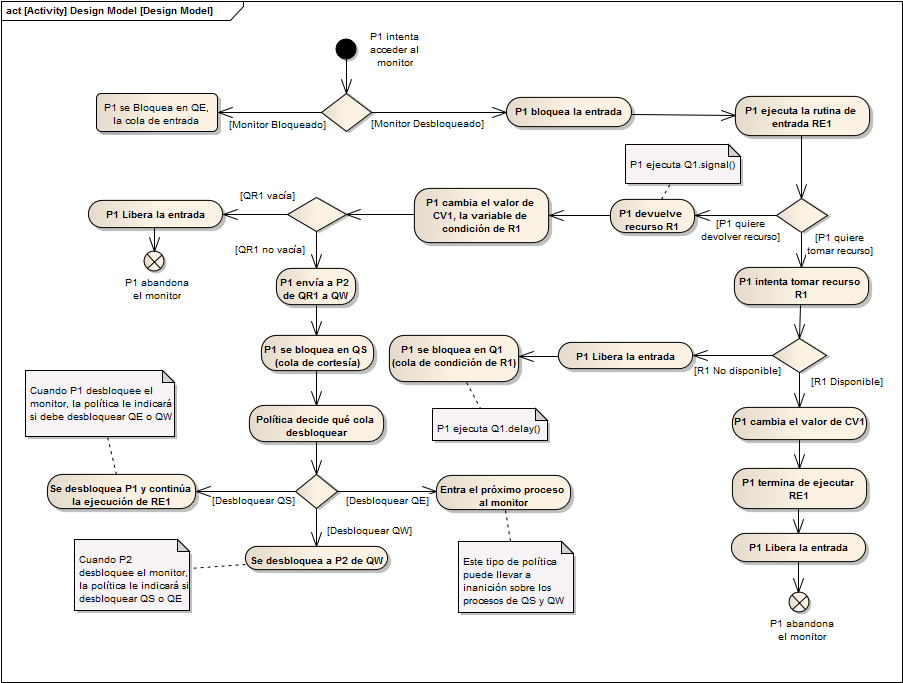
\includegraphics[width=\textwidth]{Actividad_Proceso_Monitor}
  }
  \caption{Diagrama de actividades UML de un hilo ejecutándo una rutina de
  un monitor}
  \label{fig:actividad_hilo_monitor}
\end{figure}

El diagrama de la figura \ref{fig:actividad_hilo_monitor} sugiere que un
hilo puede optar por uno de dos caminos al ejecutar una rutina del monitor:
tomar o devolver un recurso.

Existe otra opción que es tomar y devolver un recurso en la misma rutina. Este
caso no está especificado en el diagrama por simplicidad y por tratarse de una
superposición de los otros dos casos.

\subsubsection{Conclusión}
La ventaja de los monitores sobre los semáforos es que todas
las funciones de sincronización quedan confinadas dentro del monitor. De este
modo, es más sencillo verificar que la sincronización se ha realizado
correctamente y detectar los fallos. Una vez que un monitor está
correctamente programado, el acceso al recurso protegido es correcto para todos
los hilos. En el caso de los semáforos, en cambio, el acceso al recurso es
correcto sólo si \textbf{todos los hilos} que acceden al recurso están
correctamente programados.\cite{SistOpStallings} Por otro lado, las políticas
de desbloqueo permiten especificar prioridades de ejecución para los hilos,
ya sea por orden de llegada o por algún otro criterio. Un monitor diseñado de
forma modular para modificar la política brinda la posibilidad de alterar la
planificación de los hilos de acuerdo a cada caso particular. La misma
planificación resulta por demás complicada si se realiza utilizando semáforos.
Por estas razones, un punto fuerte a favor de los monitores frente a los
semáforos es la mantenibilidad del código. Por otro lado, al ser el único punto
del programa donde se toman decisiones, un monitor se convierte en un cuello de
botella para el sistema. El impacto negativo a la performance del sistema se
reduce con una arquitectura de monitores jerárquicos.
